% Setup -------------------------------

\documentclass[a4paper]{report}
\usepackage[a4paper, total={6in, 10in}]{geometry}
\setcounter{secnumdepth}{3}
\setcounter{tocdepth}{3}

\usepackage{titlepic}

\usepackage{hyperref}
\usepackage{indentfirst}

\usepackage{graphicx}
\usepackage{float}

\usepackage{enumitem}

\usepackage{minted}
\usepackage{xcolor}

\definecolor{friendlybg}{HTML}{f0f0f0}
\setminted[bash]{
	style=manni,
	bgcolor=friendlybg,
	linenos,
	frame=lines,
	framerule=0.6pt,
	framesep=5pt,
	rulecolor=orange,
	fontsize=\footnotesize
}
\setminted[dockerfile]{
	style=manni,
	bgcolor=friendlybg,
	linenos,
	frame=lines,
	framerule=0.6pt,
	framesep=5pt,
	rulecolor=orange,
	fontsize=\footnotesize
}

% Encoding
%--------------------------------------
\usepackage[T1]{fontenc}
\usepackage[utf8]{inputenc}
%--------------------------------------

% Portuguese-specific commands
%--------------------------------------
\usepackage[portuguese]{babel}
%--------------------------------------

% Hyphenation rules
%--------------------------------------
\usepackage{hyphenat}
%--------------------------------------

% Capa do relatório

\title{
    Gestão de Grandes Conjuntos de Dados
    \\ \Large{\textbf{2º Trabalho Prático}}
    \\ -
    \\ Mestrado em Engenharia Informática
    \\ Universidade do Minho
}
\author{
    \begin{tabular}{ll}
        \textbf{Grupo nº 8}
        \\
        \hline
        PG41080 & João Ribeiro Imperadeiro
        \\
        PG41081 & José Alberto Martins Boticas
        \\
        PG41091 & Nelson José Dias Teixeira
        \\
        PG41851 & Rui Miguel da Costa Meira
    \end{tabular}
    \vspace{1cm}
}

\date{\today}

\titlepic{
	\vspace{2cm}
	
\includegraphics[scale=0.065]{Images/EEUM_logo.png}
}

\begin{document}

\begin{titlepage}
    \maketitle
\end{titlepage}

% Índice

\tableofcontents
\listoffigures

% Introdução

\chapter{Introdução} \label{ch:Introduction}
\large {
    Neste trabalho prático é requerida a concretização e avaliação experimental de tarefas de armazenamento e processamento de dados através do uso da ferramenta computacional \textit{Spark} (\textit{batch} e \textit{streaming}).
    Por forma a realizar estas tarefas, são utilizados os dados públicos do \textit{IMDb}, que se encontram disponíveis em:
    \begin{center}
        \textit{\url{https://www.imdb.com/interfaces/}}
    \end{center}

    Para além destes dados, é também utilizado um gerador de \textit{streams}, baseado nos mesmos, que simula uma sequência de votos individuais de utilizadores. Este utensílio foi desenvolvido pelo docente desta unidade curricular e foi-nos disponibilizado através da plataforma \textit{Blackboard}.

    Ao longo deste documento vão também ser expostos todos os passos tomados durante a implementação das tarefas pedidas neste projeto, incluindo as decisões tomadas pelos elementos deste grupo a nível de algoritmos e parâmetros de configuração.
    Para além disso são ainda apresentadas todas as instruções que permitem executar e utilizar corretamente os programas desenvolvidos.
    Por fim, na fase final deste manuscrito, são exibidos os objetivos atingidos após a realização das tarefas propostas.
}

\chapter{Implementação} \label{ch:Implementation}
\large {
    Para a realização com sucesso deste trabalho prático, é solicitada a elaboração de três tarefas. Apresentam-se de seguida as mesmas:
    \begin{enumerate}
        \item Desenvolver uma componente de processamento de \textit{streams} que produza os seguintes resultados:
        \begin{itemize}
            \item \textbf{\textit{Log}}: armazenar todos os votos individuais recebidos, etiquetados com a hora de chegada aproximada ao minuto, em lotes de 10 minutos. Cada lote deve ser guardado num ficheiro cujo nome identifica o período de tempo;
            \item \textbf{\textit{Top3}}: exibir a cada minuto o \textit{top} 3 dos títulos que obtiveram melhor classificação média nos últimos 10 minutos;
            \item \textbf{\textit{Trending}}: apresentar a cada 15 minutos os títulos em que o número de votos recolhido nesse período sejam superiores aos votos obtidos no período anterior, independentemente do valor dos votos.
        \end{itemize}
        \item Implementar uma componente de processamento em \textit{batch} que permita realizar as seguintes tarefas:
        \begin{itemize}
            \item \textbf{\textit{Top10}}: calcular o \textit{top} 10 dos atores que participaram em mais títulos diferentes;
            \item \textbf{\textit{Friends}}: computar o conjunto de colaboradores de cada ator (i.e., outros atores que participaram nos mesmos títulos);
            \item \textbf{\textit{Ratings}}: atualizar o ficheiro \textsl{"title.ratings.tsv"} tendo em conta o seu conteúdo anterior e os novos votos recebidos até ao momento.
        \end{itemize}
        \item Escolher a configuração e a implementação que, para o mesmo \textit{hardware}, permite receber e tratar o maior débito de eventos. Esta tomada de decisão deve ser devidamente justificada com recurso a resultados experimentais.
    \end{enumerate}
    
    Nas próximas secções são expostas as implementações para cada uma destas tarefas bem como algumas sugestões alternativas que poderiam ser tomadas em consideração.

    \section{Configuração} \label{sec:Configuration}
        Nesta secção do relatório são apresentadas as configurações relativas ao arranque do \textit{cluster}, instanciando-se tanto as respetivas entidades (\textsl{master}, \textsl{worker1} e \textsl{worker2}) como as máquinas virtuais pertencentes à plataforma \textit{Google Cloud}, e, ainda, a configuração genérica para a execução individual de cada exercício proposto. 

        \subsection{Arranque do \textit{cluster}} \label{subsec:Configuration-Cluster}
            A configuração escolhida para a realização deste projeto coincide com a que foi sugerida pelo docente desta unidade curricular, isto é, o \textbf{\textit{docker swarm}}.
            Esta configuração permite não só tirar partido da ferramenta computacional \textit{Google Cloud} como também possibilita o uso de plataformas como o \textit{Hadoop HDFS} e o \textit{Apache Spark}.
            Como seria de esperar, todos os ficheiros de \textit{input} utilizados para atingir os objetivos traçados neste trabalho prático são armazenados no sistema \textit{Hadoop HDFS}.
            
            Exibe-se de seguida todos os passos de configuração associados ao \textit{docker swarm}:
            \begin{enumerate}[label=\textbf{\arabic*.}]
                \item criação das instâncias relativas às 3 entidades intrínsecas à arquitetura do sistema, isto é, as entidades \textsl{master}, \textsl{worker1} e \textsl{worker2}:
                \begin{figure}[H]
                    \centering
                    \begin{minted}{bash}
docker-machine create \
               --driver google --google-project ferrous-aleph-271712 \
               --google-zone europe-west1-b \
               --google-machine-type n1-standard-4 \
               --google-disk-size=100 \
               --google-disk-type=pd-ssd \
               --google-machine-image \
       https://www.googleapis.com/compute/v1/projects/centos-cloud/global/images/centos-7-v20200309 \
               master
                    \end{minted}
                    \vspace{-5mm}
                    \caption{Configuração - Criação da instância associada à entidade \textsl{master}}
                    \label{fig:1}
                \end{figure}
                
                \begin{figure}[H]
                    \centering
                    \begin{minted}{bash}
docker-machine create \
               --driver google --google-project ferrous-aleph-271712 \
               --google-zone europe-west1-b \
               --google-machine-type n1-standard-4 \
               --google-disk-size=100 \
               --google-disk-type=pd-ssd \
               --google-machine-image \
       https://www.googleapis.com/compute/v1/projects/centos-cloud/global/images/centos-7-v20200309 \
               workerName
                    \end{minted}
                    \vspace{-5mm}
                    \caption{Configuração - Criação de uma instância \textsl{worker}}
                    \label{fig:2}
                \end{figure}

                De salientar que a designação \texttt{ferrous-aleph-271712} corresponde ao identificador do projeto presente na plataforma \textit{Google Cloud} de um dos elementos que compõem este grupo.
                Assim, esta denominação deve ser substituída pelo nome do projeto do utilizador. Relativamente à designação \textit{workerName}, esta deve ser subtituída pelos nomes das entidades \textit{worker} referidas no ponto acima (\textsl{worker1} e \textsl{worker2}).

                \item configuração do \textit{swarm} relativo às entidades \textsl{master}, \textsl{worker1} e \textsl{worker2}:
                \begin{figure}[H]
                    \centering
                    \begin{minted}{bash}
docker-machine ssh master sudo docker swarm init
                    \end{minted}
                    \vspace{-5mm}
                    \caption{Configuração - \textit{swarm} \textsl{master}}
                    \label{fig:4}
                \end{figure}

                \begin{figure}[H]
                    \centering
                    \begin{minted}{bash}
docker-machine ssh workerName sudo docker swarm join --token \
               SWMTKN-1-5zfy2iio54tma997pnt96gq5095fimqn2hxr2a8j16ogq0n3c9-0kp6mi5iuj956gpl9sfccd5bo\
               10.132.0.8:2377
                    \end{minted}
                    \vspace{-5mm}
                    \caption{Configuração - \textit{swarm} \textsl{worker}}
                    \label{fig:5}
                \end{figure}

                \item ativação do ambiente da entidade \textsl{master}:
                \begin{figure}[H]
                    \centering
                    \begin{minted}{bash}
docker-machine env master
eval $(docker-machine env master)
                    \end{minted}
                    \vspace{-5mm}
                    \caption{Configuração - Ativação do ambiente da entidade \textsl{master}}
                    \label{fig:7}
                \end{figure}

                \item compilação do gerador de \textit{streams}, isto é, o \textit{streamgen}:
                \begin{figure}[H]
                    \centering
                    \begin{minted}{bash}
mvn package
docker build -t streamgen .
                    \end{minted}
                    \vspace{-5mm}
                    \caption{Configuração - Compilação do utensílio \textit{streamgen}}
                    \label{fig:9}
                \end{figure}

                \item arranque do sistema com a configuração \textit{swarm} especificada:
                \begin{figure}[H]
                    \centering
                    \begin{minted}{bash}
docker stack deploy -c ../swarm-spark/docker-compose.yml mystack
                    \end{minted}
                    \vspace{-5mm}
                    \caption{Configuração - Arranque do sistema}
                    \label{fig:10}
                \end{figure}

                É de realçar que no ficheiro \textit{"docker-compose.yml"} encontra-se uma configuração \textit{docker} semelhante à que foi utilizada no guião nº 8 desta unidade curricular.
                A única diferença presente no mesmo diz respeito à integração do gerador de \textit{streams} (\textit{streamgen}) desenvolvido pelo docente como um \textit{container docker} do sistema.
                Assim, no momento do arranque do sistema, a ferramenta \textit{streamgen} é convenientemente invocada, ficando à espera de novas conexões por parte dos utilizadores.
                Apresenta-se de seguida a configuração presente no ficheiro \textit{"docker-compose.yml"} relativa ao \textit{streamgen}:

                \begin{figure}[H]
                    \centering
                    \begin{minted}{bash}
streamgen:
    image: streamgen
    command: hdfs:///data/title.ratings.tsv 120
    env_file:
        - ./hadoop.env
    deploy:
        mode: replicated
        replicas: 1
        placement:
            constraints:
                - "node.role==manager"
                    \end{minted}
                    \vspace{-5mm}
                    \caption{Configuração - Ficheiro \textit{"docker-compose.yml"} - \textit{streamgen}}
                    \label{fig:11}
                \end{figure}


                \item acesso à plataforma \textit{Hadoop HDFS} por parte do utilizador:
                \begin{figure}[H]
                    \centering
                    \begin{minted}{bash}
docker run --network mystack_default --env-file ../swarm-spark/hadoop.env -it bde2020/hadoop-base \
       bash
                    \end{minted}
                    \vspace{-5mm}
                    \caption{Configuração - Acesso à plataforma \textit{Hadoop HDFS}}
                    \label{fig:13}
                \end{figure}
            \end{enumerate}}

            Com a concretização dos 6 passos descritos acima, fica concluída a configuração do \textit{docker swarm}.
        
        \subsection{Execução de tarefas} \label{subsec:Configuration-Dockerfile}
            Para a execução dos 3 exercícios descritos na \hyperref[ch:Implementation]{secção} relativa à implementação, é disponibilizado um ficheiro com a designação \textit{Dockerfile}.
            Neste é especificado o nome da classe relativa à proposta que se presente executar, procedendo corretamente à sua invocação.
            Como tal, em primeiro lugar é preciso desempenhar a seguinte instrução:
            \begin{figure}[H]
                \centering
                \begin{minted}{bash}
mvn package
                \end{minted}
                \vspace{-5mm}
                \caption{Configuração - Obtenção do ficheiro \textit{jar} do projeto}
                \label{fig:14}
            \end{figure}
            
            De seguida, invoca-se o \textit{dockerfile} em causa. Expõe-se agora o seu conteúdo:
            \begin{figure}[H]
                \centering
                \begin{minted}{dockerfile}
FROM bde2020/spark-base:2.4.4-hadoop2.7
COPY target/TP2-1.0-SNAPSHOT.jar /
ENTRYPOINT ["/spark/bin/spark-submit", "--class", "package.className", "--master", \
            "spark://spark-master:7077", "/TP2-1.0-SNAPSHOT.jar"]
                \end{minted}
                \vspace{-5mm}
                \caption{Configuração - \textit{Dockerfile}}
                \label{fig:15}
            \end{figure}

            A este ficheiro estão associadas alguma opções de execução que garantem uma comunicação fidedigna com o sistema inicialmente declarado. Eis as mesmas:
            \begin{figure}[H]
                \centering
                \begin{minted}{bash}
-p 4040:4040 --network mystack_default --env-file ../swarm-spark/hadoop.env
                \end{minted}
                \vspace{-5mm}
                \caption{Configuração - Opções de execução do ficheiro \textit{Dockerfile}}
                \label{fig:16}
            \end{figure}

            De salientar que é escolhida a opção \textsl{master} no campo relativo ao \textit{docker machine} para, mais uma vez, garantir uma configuração válida do sistema em causa.

    \section{1ª Tarefa} \label{sec:Task1}
        Na 1ª tarefa deste projeto é pedido o desenvolvimento de uma componente de processamento de \textit{streams}. Nesta é solicitada a realização de vários exercícios com diferentes caraterísticas. Como tal, apresenta-se de seguida as respetivas implementações e, ainda, possíveis alternativas nas suas concretizações.

        \subsection{\textit{Log}} \label{subsec:Task1-Log}
            Neste exercício, tal como foi indicado no início deste \hyperref[ch:Implementation]{capítulo}, é imposto o armazenamento de todos os votos individuais recebidos com a indicação da hora de chegada aproximada ao minuto, em lotes de 10 minutos, sendo que cada lote é guardado com o nome relativo ao período de tempo em causa.

            Dito isto, para proceder ao tratamento da aproximação da hora recebida ao minuto, foi implementada uma função para o efeito. Optou-se por não só guardar a hora referida como também a data em questão, exibindo, desta forma, um maior detalhe da informação recebida.
            Uma vez implementada esta função, foi utilizado o método \textit{transform} que faz uso da noção de tempo. Com esta vertente, é possível associar a cada \textit{RDD} do conjunto de dados a hora, aproximada ao minuto, em que este foi processado.

            Por fim, com os aspetos computacionais mencionados acima, resta armazenar os dados recebidos pela ferramenta \textit{streamgen} com recurso à definição de uma janela com 10 minutos de duração e 10 minutos de deslocamento.
            Os \textit{RDD}'s em causa são guardados na diretoria \texttt{Log/Lot\{\textit{i}\} - dd-MM-yyyy HH-mm}, sendo que \texttt{i} diz respeito ao número do lote (que começa no número 1 e que é constamente incrementado) e \texttt{dd-MM-yyyy HH-mm} refere-se ao padrão do período temporal.
            
            De maneira a guardar apenas um ficheiro (\textit{part-00000}), a todos os \textit{RDD}'s resultantes foi aplicado o método \textit{coalesce(1)}.
            Esta última função, quando comparada com a \textit{repartition()}, não necessita de efetuar um \textit{shuffle} completo dos dados.
            Para além disto, esta abordagem foi considerada nesta implementação dado que no exercício \textit{Ratings} (\textit{batch}) será necessário realizar a leitura do ficheiro mencionado. 
            Consequentemente, em vez de operar várias leituras de ficheiros, efetua-se apenas uma leitura, permitindo, assim, uma maior eficiência.

        \subsection{\textit{Top3}} \label{subsec:Task1-Top3}
            Para este exercício é necessário recolher os novos votos e calcular as classificações médias dos últimos dez minutos, a cada minuto.

            De forma a recolher e tratar os novos votos gerados pelo \textit{streamgen}, mapeia-se cada um dos mesmos para um par em que a chave é o identificador do filme e o valor um outro par: o voto e o número 1.
            
            Desta forma, é possível, depois, utilizar o método \textit{reduceByKeyAndWindow}, de forma a que, para a duração (10) e deslizamento (1) definidos para a janela, seja possível realizar as operações necessárias.
            Com o método anterior, é possível definir duas funções para aplicar aquando do deslizamento da janela, agrupando previamente os dados pela sua chave (identificador do filme): a primeira diz respeito ao que fazer com os novos dados que chegam (novos votos) e a segunda diz respeito ao que fazer com os dados que deixam de ficar dentro da duração da janela (votos de há mais de dez minutos).
            
            Dito isto, a primeira função deve somar ambos os componentes do par gerado (voto, 1), por forma a obter um novo par com a soma total dos votos e o número total de votos, para cada filme.
            A segunda função deverá subtrair os mesmos, de forma a que o votos gerados há mais de dez minutos deixem de ter influência nos resultados.
            
            Por fim, mapeiam-se os resultados para um par em que a chave mantém o identificador do filme e o valor passa a ser a divisão entre os componentes do par que representava o valor anteriormente.
            Assim, o novo par associará a classificação média dos últimos dez minutos ao identificador do filme.

            Os últimos passos serão juntar os resultados da computação anterior com uma primeira computação que extrai os títulos dos filmes do ficheiro "\textit{title.basics.tsv}" \hspace{0.1mm} e os associa ao seu identificador. Por fim, são exibidos os resultados obtidos.
            A junção implica o uso do método \textit{transformToPair} de forma a que se proceda à junção de cada \textit{RDD}, resultante do processamento de \textit{stream} explicado acima, ao \textit{JavaPairRDD} explicado anteriormente.

            Ao resultado desta junção aplica-se o método \textit{forEachRDD} e calcula-se, com o método \textit{top}, os 3 filmes com melhor classificação média.
            Para isso foi necessário explicitar um novo comparador, uma vez que o tipo de dados \textit{Tuple2} não é serializável.
            Por fim, imprime-se o resultado. Esta impressão deve ocorrer uma vez a cada minuto.

        \subsection{\textit{Trending}} \label{subsec:Task1-Trending}
            O último exercício da primeira tarefa foi talvez o mais desafiante de todos, pelo facto de ser necessário comparar os novos dados com dados anteriores.
            Para resolver o problema, foi decisivo o uso do método \textit{mapWithState}.

            Começou-se da forma mais simples, retirando-se as informações pertinentes do ficheiro "\textsl{title.basics.tsv}", para mais tarde serem usadas.

            Passando ao processamento de \textit{stream}, este, inicialmente, foi muito semelhante ao do exercício anterior, sendo que, em vez de um par associado ao identificador do filme, foi apenas associado o inteiro 1.
            Desta forma, cada voto terá o mesmo peso, como é exigido, já que se querem comparar números de votos e não classificações.
            O método \textit{reduceByKeyAndWindow} foi aplicado da mesma forma que no exercício anterior, com a alteração dos valores de duração e deslizamento da janela, agora 15 em ambos os casos.

            A diferença marca-se depois, com o \textit{output} gerado anteriormente a alimentar o método \textit{mapWithState}, por forma a ser possível comparar os dados (votos) dos últimos 15 minutos com os gerados nos 15 minutos anteriores a estes.
            Neste último método, opera-se sobre um três variáveis: a chave \texttt{k}, o novo valor \texttt{v} (pode existir ou não) e o estado anterior \texttt{s} (pode existir ou não; representa a quantidade de votos dos 15 minutos anteriores aos em questão). 
            É declarada uma variável booleana \texttt{trending}. Se \texttt{v} não existir, \texttt{trending} passa a \textit{false} e o estado \texttt{s} é apagado. 
            Se \texttt{v} existir mas \texttt{s} não existir, então \texttt{trending} passa a \textit{true} e \texttt{s} assume o valor de \texttt{v}.
            Caso existam as duas variáveis, então as mesmas são comparadas e \texttt{trending} fica com o resultado dessa comparação (\texttt{v} > \texttt{s}). 
            Independentemente do resultado desta última comparação, \texttt{s} assume o valor de \texttt{v}.
            Por fim, é retornado um par que associa \texttt{trending} à chave \texttt{k}.

            De forma a simplificar a junção desta informação com a retirada do ficheiro "\textsl{title.basics.tsv}", é ainda executado o método \textit{mapToPair}, de forma a que o resultado de toda esta computação seja um \textit{JavaPairDStream}.

            Posteriormente, segue-se à junção das informações. Para isto, procede-se da mesma forma que no exercício anterior, sendo que ainda se aplica uma filtragem aos \textit{RDD}'s que tenham os valores de \texttt{trending} a falso.
            Assim, teremos apenas os filmes que estão \textit{trending}, ou seja, que tiveram mais votos no último período de 15 minutos, quando comparados com o período anterior.
            Por último, antes de imprimir, procede-se ainda ao mapeamento do resultado anterior, de forma a descartar os identificadores dos filmes e os valores booleanos, ficando-se apenas com os nomes dos filmes que estão em alta.

            Resta então apenas a impressão desses nomes. Para isso, aplica-se o método \textit{forEachRDD} ao resultado da execução anterior e aplica-se o método \textit{collect} a cada \textit{RDD}.


    \section{2ª Tarefa} \label{sec:Task2}
        Na 2ª tarefa deste trabalho prático é proposta a implementação de uma componente de processamento em \textit{batch}. Nesta é solicitada a realização de 3 exercícios com diferentes caraterísticas e, como tal, foram adotapadas abordagens distintas para cada um deles.
        Divulgam-se, de seguida, as respetivas implementações.

        \subsection{\textit{Top10}} \label{subsec:Task2-Top10}
            Nesta subtarefa é pedido o cálculo dos 10 atores que participaram em mais filmes distintos.
            Ênfase para distintos, uma vez que, no caso das séries, muitos dos episódios apresentam o nome da série, o que poderia levar a um erro na implementação caso estes fossem tomados em conta.

            Durante o processamento inicial do ficheiro \textsl{"title.principals.tsv"} é, tal como seria de esperar, ignorado o respetivo cabeçalho.
            Posteriormente, é extraída, linha após linha, a informação pertinente do mesmo, isto é, os identificadores do filme e do ator em questão, agrupando os dados pela segunda componente. 
            Esta última ação é efetuada com recurso à chamada do método \textit{groupByKey}.
            Com esta computação, obtém-se para cada ator a lista de filmes em que este participou.
            Atendendo ao resultado exigido neste exercício, basta, nesta etapa do processamento, efetuar a contagem dos filmes associados a cada ator.
            Para tal, mapeia-se o resultado da agregação anterior de forma a associar a cada ator, o número de filmes em que o mesmo participou.
            Por razões de ordenação e seleção dos atores mais ativos, trocou-se a ordem mencionada acima, sendo que, desta forma, temos o número de filmes como chave e o identificador do ator como valor.

            A recolha dos 10 atores que participaram em mais filmes é finalizada com a chamada do método \textit{top}. Esta função permite extrair os \textit{k} maiores registos de um \textit{RDD}, segundo uma determinada ordem.
            Para este exercício, houve a necessidade de implementar um comparador explícito, numa classe à parte, dado que o tipo de dados \textit{Tuple2} não é, por definição, serializável.

            \begin{figure}[H]
                \centering
                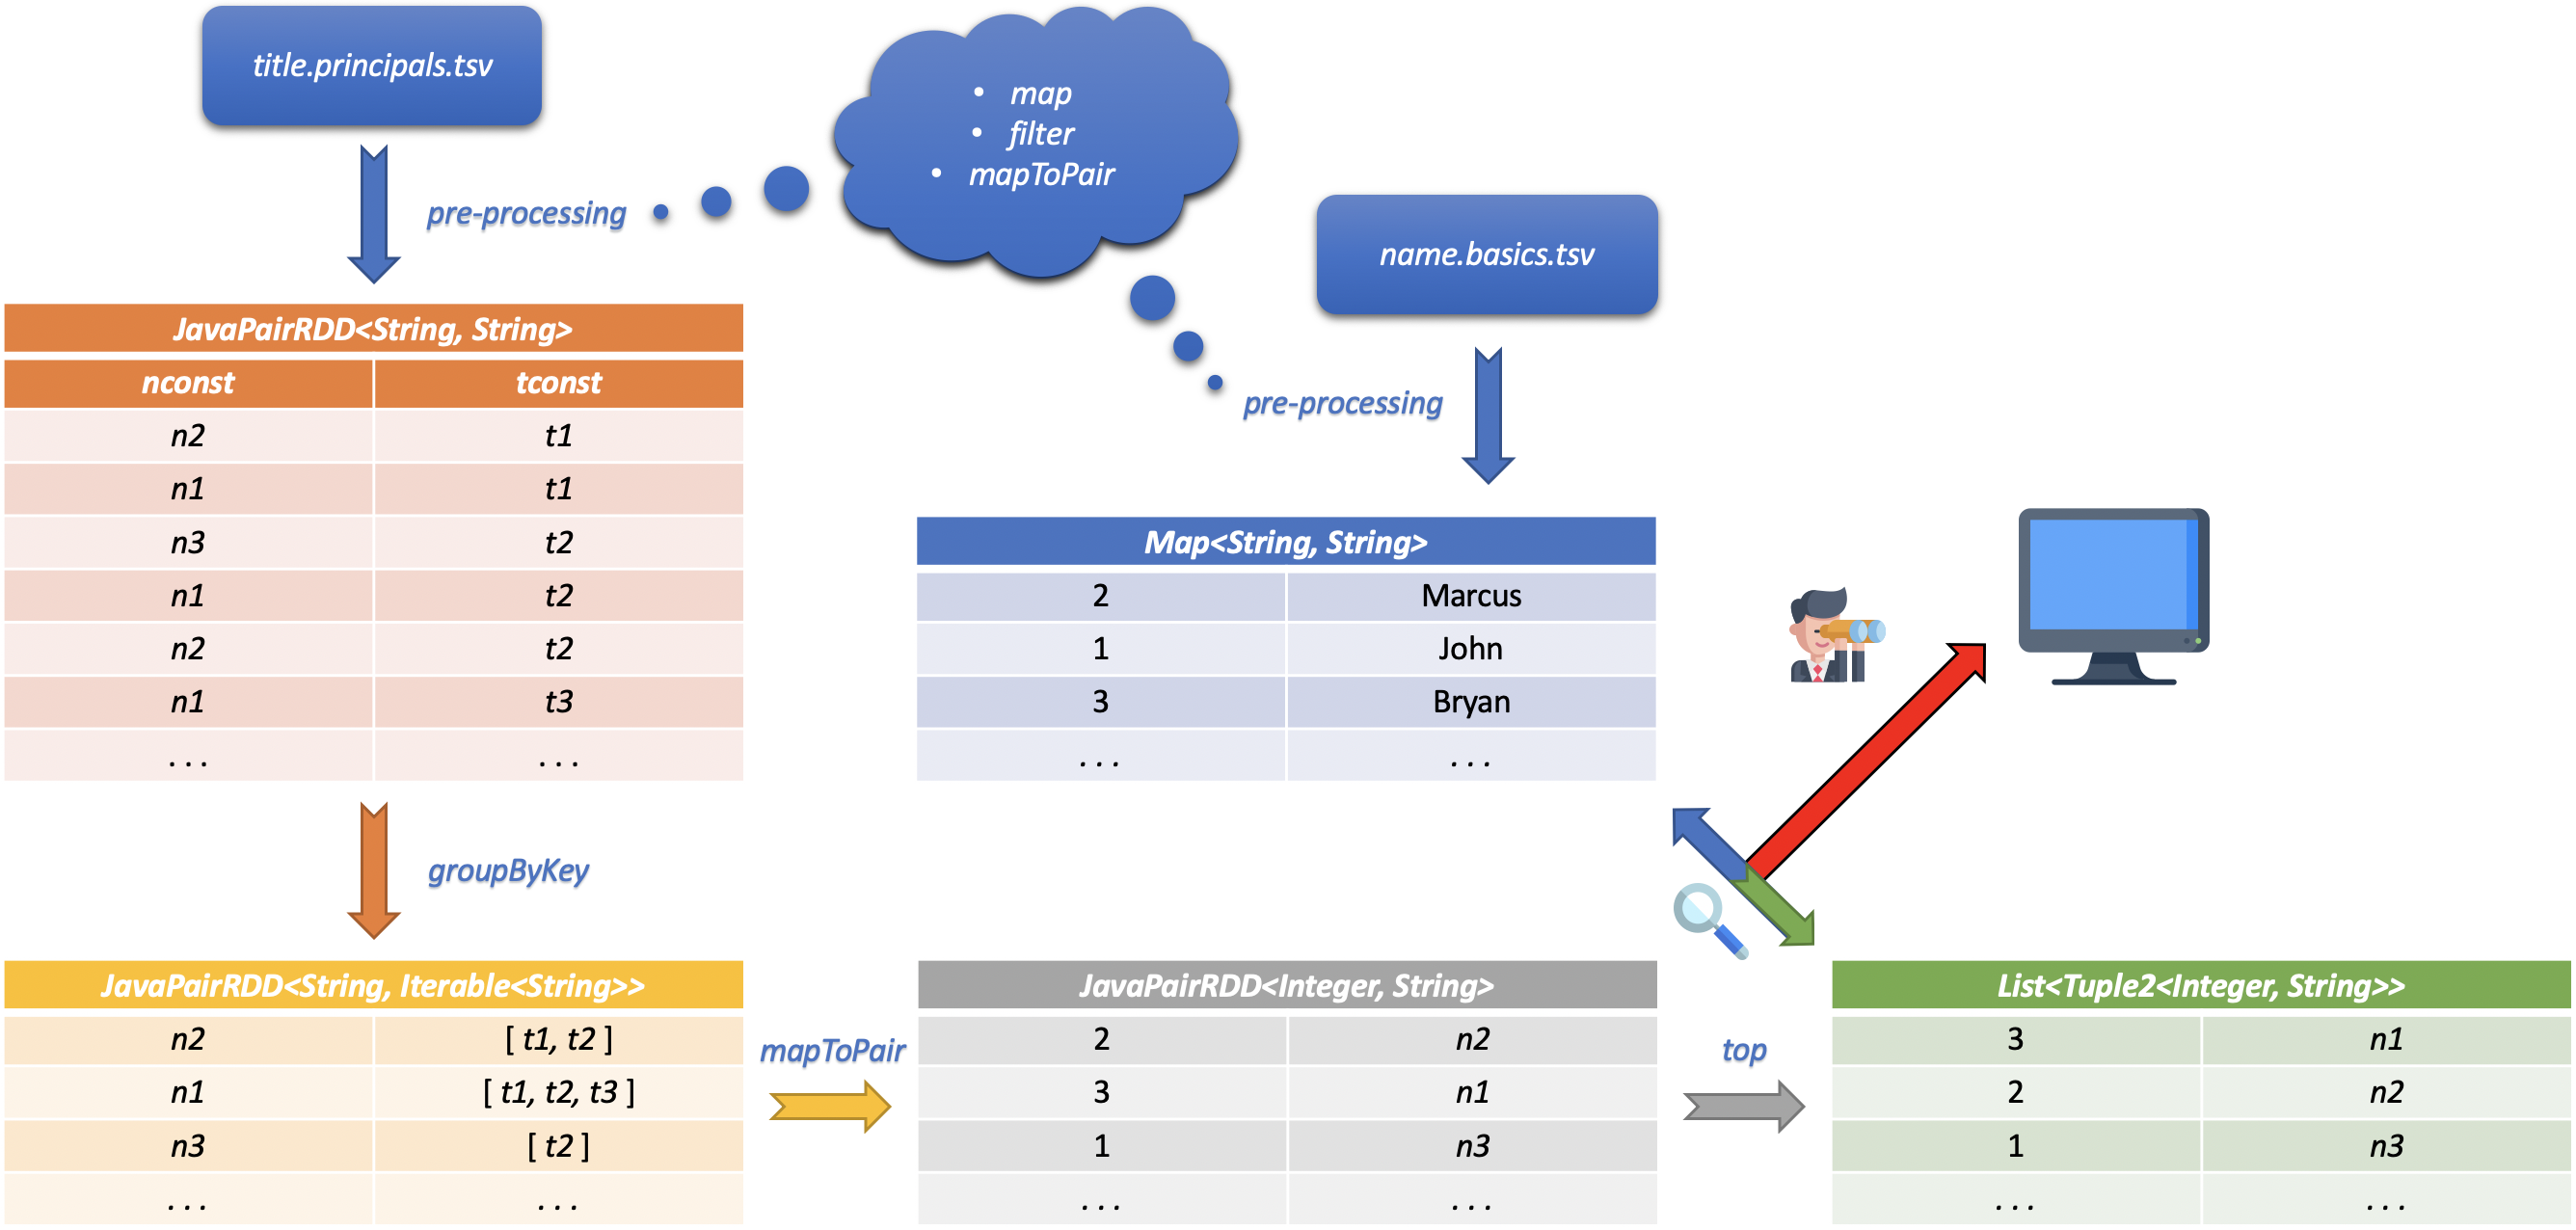
\includegraphics[width=1.0\textwidth]{Images/Task 2 - Top10.png}
                \caption{2ª Tarefa (\textit{batch}) - Esquema do processamento relativo à subtarefa \textit{Top10}}
                \label{fig:17}
            \end{figure}

            \subsubsection{Alternativa} \label{sssec:Task2-Top10-Alternativa}
                Uma forma alternativa de resolver este exercício seria, na última fase do processamento, utilizar o método \textit{take} em detrimento da função \textit{top}.
                Esta escolha não foi tomada em consideração na implementação uma vez que o primeiro método necessita previamente que a informação esteja devidamente ordenada.
                Esta ordenação teria de ser realizada com a invocação do método \textit{sortByKey(false)}, colocando a contagem dos filmes em que cada ator participou de forma decrescente.
                Este último facto representa uma ineficiência no cálculo do resultado pretendido uma vez que é efetuada a ordenação completa da informação em causa e, para além disso, realiza-se desnecessariamente um passo computacional extra.

        \subsection{\textit{Friends}} \label{subsec:Task2-Friends}
            Neste exercício é requerido a computação do conjunto de colaboradores associado a cada ator, ou seja, o grupo dos atores que particapam nos mesmos filmes.
                
            Durante o processamento inicial do ficheiro \textsl{"title.principals.tsv"} é, tal como seria de esperar, ignorado o respetivo cabeçalho.
            Posteriormente, é extraída, linha após linha, a informação pertinente do mesmo, isto é, os identificadores do filme e do ator em questão, agrupando os dados pela primeira componente. Esta última ação é efetuada com recurso à chamada do método \textit{groupByKey}.

            De forma a obter o resultado solicitado nesta subtarefa, é necessário, nesta fase da computação, proceder à realização de uma operação denominada por produto cartesiano. 
            Nesta operação computa-se, num dado momento, todos os pares dos atores que colaboraram num determinado filme, passando a existir apenas pares de atores, com a chave a representar um ator e o valor um dos seus colaboradores.
            De realçar que estes pares são guardados num \textit{Set}, de forma a eliminar repetições.

            Uma vez realizado este cálculo, é invocado novamente o método \textit{groupByKey} de forma a obter o resultado pretendido, isto é, o conjunto de colaboradores para cada ator.

            \begin{figure}[H]
                \centering
                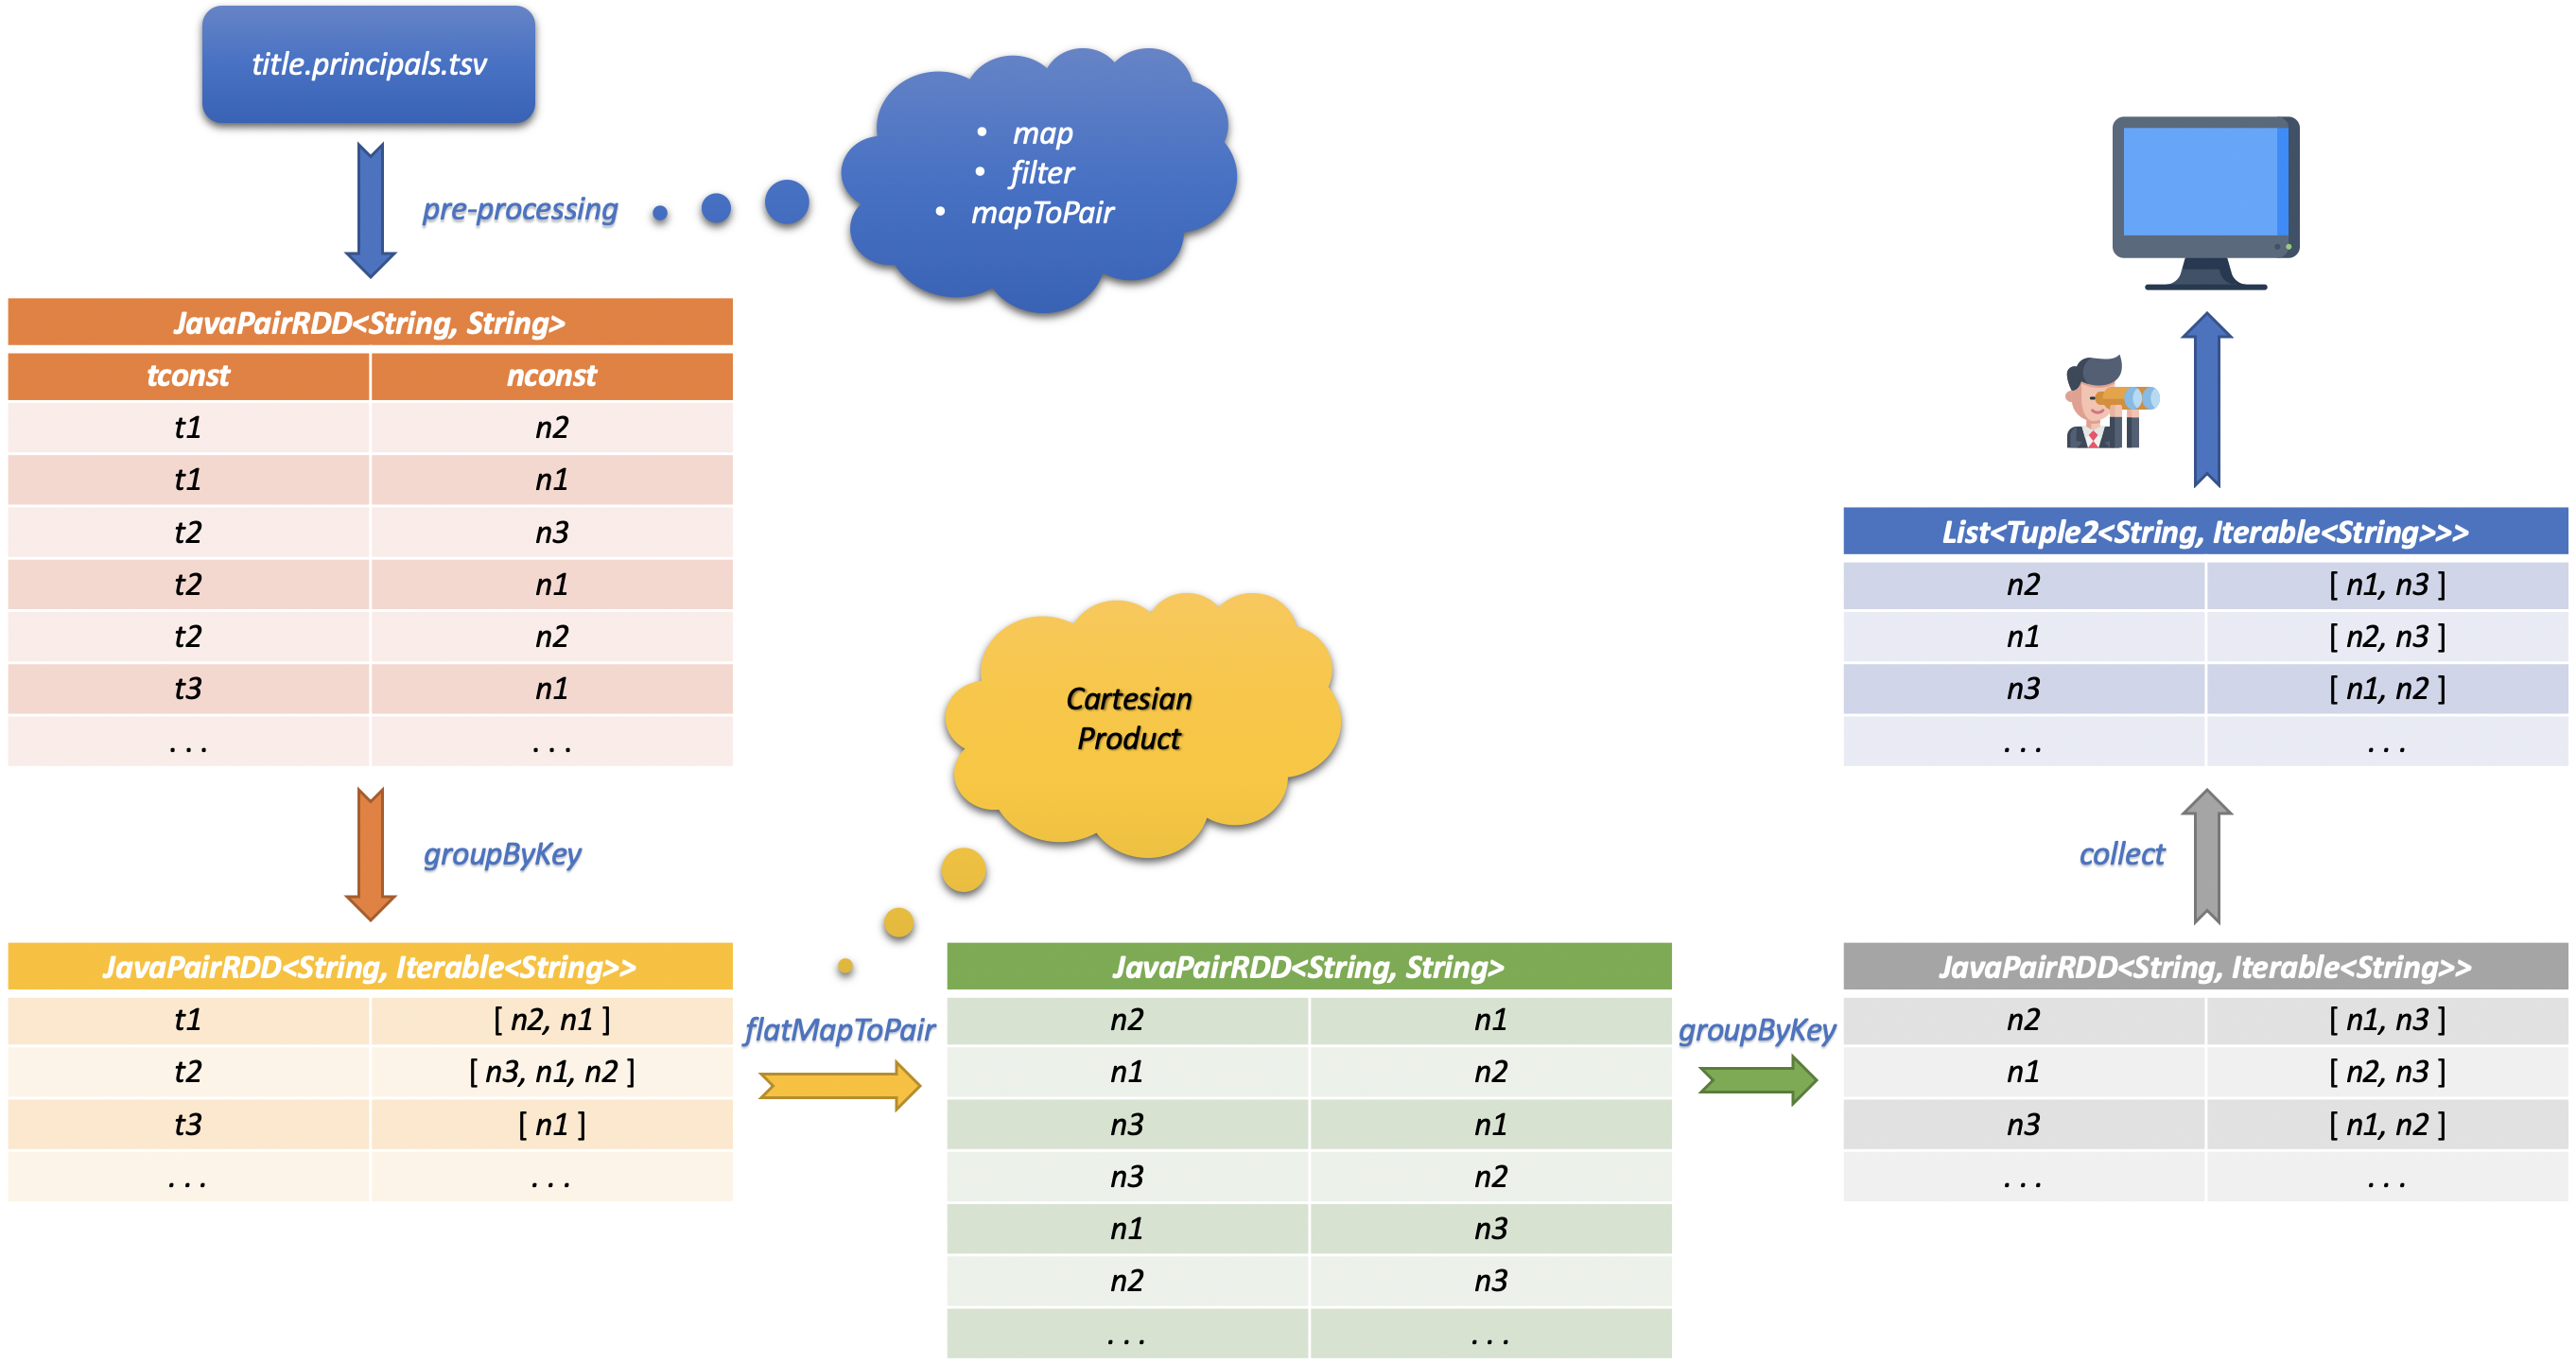
\includegraphics[width=1.0\textwidth]{Images/Task 2 - Friends.png}
                \caption{2ª Tarefa (\textit{batch}) - Esquema do processamento relativo à subtarefa \textit{Friends}}
                \label{fig:18}
            \end{figure}

        \subsection{\textit{Ratings}} \label{subsec:Task2-Ratings}
            Este último exercício da segunda tarefa divide-se em três fases, tratar os votos, aplicar as alterações provocadas pelos mesmos e, por fim, atualizar o ficheiro "\textsl{title.ratings.tsv}".

            Assim, foram desenvolvidas duas funções auxiliares: 
            a primeira trata de coletar os votos apresentados nos ficheiros de \textit{Log} produzidos pelo primeiro exercício da primeira tarefa, passando-os para um novo ficheiro de texto; 
            a segunda atualiza o ficheiro "\textsl{title.ratings.tsv}", gerando um novo, "\textsl{title.ratings.tsv.new}".

            A função principal começa por a primeira das funções descritas anteriormente.

            De seguida, carrega as informações de \textit{rating} dos filmes, aplicando-lhe a filtragem que permite remover o cabeçalho.
            A isto, aplica uma alteração, com recurso ao método \textit{mapToPair}, de forma a guardar apenas o identificador do filme associado ao par: multiplicação entre a classificação média obtida até agora e o número total de votos; número total de votos.
            Esta multiplicação permite obter uma aproximação da soma de todos os votos, útil para calcular a nova classificação média.

            Posto isto, passa-se à fase de carregar os novos votos, por forma a concretizar as alterações necessárias.
            Utilizando o método \textit{textfile} do \texttt{JavaSparkContext}, é possível ler e manipular o ficheiro de texto gerado pela primeira função auxiliar, como mencionado anteriormente.
            Assim, carregam-se os novos votos, agrupando os mesmos por identificador do filme. Deste modo, obtém-se, para cada filme, uma lista de todos os novos votos.
            A este resultado, é aplicada uma última transformação: gera-se um par com a soma de todos os votos e o número total de votos. Este par fica associado ao identificador do filme.

            De forma a cruzar as informações dos novos votos com as médias já existentes, é realizado um \textit{left outer join}.
            Desta operação obtemos, associado ao identificador de um filme, os valores extraídos na primeira fase e os valores extraídos na segunda, caso existam.
            De seguida, somam-se os valores da soma total dos votos e do número total de votos, obtendo-se um par com os novos totais associado ao identificador do filme correspondente.
            De realçar que, para os filmes que não tiveram novos votos, não é feita esta operação, manténdo-se os valores iniciais.

            Por fim, é dividida a soma total dos votos pelo número total de votos, de forma a obter-se a nova classificação média, sendo que se preserva o número total de votos.
            É ainda aplicado o método \textit{map}, no sentido de cada par ser convertido numa \textit{string} que irá ser uma linha do novo ficheiro.

            A última etapa passa por guardar todas as alterações, pelo que é chamada a segunda das funções descritas acima.
            Esta função trata de criar um novo ficheiro, "\textsl{title.ratings.tsv.new}", onde guarda todos os filmes e respetivos classificações e número de votos, mantendo o formato do ficheiro anterior.


    \section{3ª Tarefa} \label{sec:Task3}
    Para esta tarefa foram realizados alguns testes, com diferentes configurações, de forma a se perceber qual delas permitia o melhor desempenho.
    Os testes foram efetuados em máquinas com 4 CPUs e 15 GiB de memória.

    Para o caso da primeira tarefa (\textit{stream}) observou-se o uso dos recursos computacionais, sendo que, tanto o uso de CPU como de memória se mantiveram reduzidos.
    Assim, tudo indica que o uso de apenas 1 CPU e 2 GiB de memória deverão ser suficientes.
    De realçar que, para este caso, foi testado o exercício Top3.

    Para o caso da segunda tarefa (\textit{batch}), o tempo de execução foi o critério de desempate.
    Foi testado o exercício Top10, sendo que o aumento de memória não teve efeito no tempo de execução, pelo que um mínimo de 2 GiB de memória deverão ser necessários.
    Quanto aos CPUs, os resultados já foram distintos. O uso de um maior número de CPUs traduziu-se num melhor desempenho. Portanto, o uso dos 4 CPUs disponíveis é aconselhado.
    
    Para além deste exercício testou-se ainda, para a segunda tarefa, o exercício \textit{Friends}. 
    Neste caso, a memória parece ter impacto no tempo de execução, pelo que se aconselha o uso de, pelo menos, 8 GiB de memória para este exercício.

    Também foi testado o impacto do tamanho dos blocos de memória aquando do carregamento, para o sistema HDFS, dos diferentes ficheiros utilizados.
    Estes últimos testes indicaram que o tamanho dos blocos de memória não têm grande influência na execução dos algoritmos desenvolvidos.


\chapter{Conclusão} \label{ch:Conclusion}
\large{
    
}

\appendix
\chapter{Observações} \label{ch:Observations}
\begin{itemize}
    \item Documentação \textit{Java} 8:
    \par \textit{\url{https://docs.oracle.com/javase/8/docs/api/}}
    \item \textit{Maven}:
    \par \textit{\url{https://maven.apache.org/}}
    \item \textit{Docker}:
    \par \textit{\url{https://www.docker.com/}}
    \item \textit{Apache Spark}:
    \par \textit{\url{https://spark.apache.org/}}
    \item \textit{Apache Hadoop}:
    \par \textit{\url{http://hadoop.apache.org/}}
\end{itemize}

\end{document}